\documentclass[11pt]{article}
\usepackage[margin=0.85in]{geometry}
\usepackage{graphicx}
\usepackage{amsmath}
\usepackage[colorlinks=true,urlcolor=blue]{hyperref}
\usepackage{booktabs}
\begin{document}
\section*{Certified n51 polynomial-01 D4 bound}
The original independent checker accepted all 52 multiplication conditions for
the frozen n51 polynomial-01 input. It verified $1\notin W_4(F)$ and
$\operatorname{codim}W_4(F)\geq45{,}615$; fresh exact enumeration found zero
Boolean solutions. Therefore the last fall degree of this named presentation
is at least five. The degree-four certificate has 1,680,493,280 bytes;
its SHA-256 is recorded in \texttt{evidence/result.json}.
The producer and checker recorded 3,191.971 and 1,282.693 seconds respectively
on the shared host; these are L0 execution records.

\section*{Next-degree resource profile}
The retained D4 certificate yields 103,877 working coordinates and 58,262
border coordinates for the bounded D5 representation. Its source-derived
allocation envelope at chunk size 60,000 is 64,677,063,002 bytes. Polynomial-00
has 103,867 working coordinates and a 64,638,795,838-byte envelope. These
are allocation calculations, not measured peak memory or D5 results.

\begin{center}
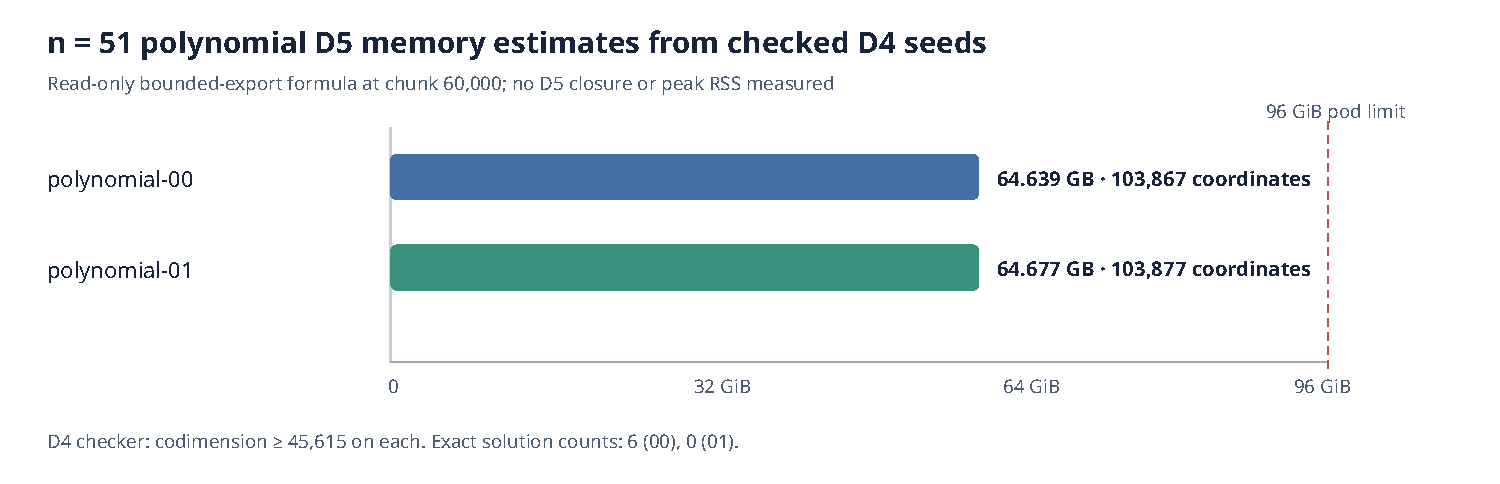
\includegraphics[width=\linewidth]{capacity.pdf}
\end{center}

\noindent The companion Markdown report links the raw result, checker output,
profile, small-file manifest, and public archive acknowledgement.
\end{document}
